\documentclass{article}

\usepackage{packages}
\usepackage{environments}
\usepackage{commands}

\begin{document}

\title{Typing Analysis}
\author{Dima Trushin}
\date{}
	
\maketitle
\tableofcontents

\section{General information}

The application uses Qt environment as an ecosystem. It does not use RTTI but uses exceptions. All components of the program must be inside NSApplication namespace. Nested namespaces should be placed in a subfolder of the project.

\subsection{Addressable objects}

I use term addressable object. It means an object that can be referenced by other objects. There are several types of addressable objects:
\begin{enumerate}
\item QObject
\item CApplicationImpl
\item Observer/Observable (TO DO)
\end{enumerate}
Addressable objects must be created on heap via \verb"std::make_unique" or similar mechanism. An exception to this rule: you may create an addressable object inside another addressable object.

\subsection{Exceptions}

The strategy is to catch exception, show a message, and die. Since Qt environment is not totally exception safe, it is not allowed to throw exceptions in an event loop. If a QObject requires to throw an exception and terminate the program it catches the exception by itself and then sends a signal to CQtLoopException object. CQtLoopException shows a message and stops the event loop. CQtLoopException is a singleton, it uses CAnyGlobalAccess template (see~\ref{section::Singleton}).

\section{Application Structure}

\subsection{Overview}

CApplication object initialize all required resources for the application including the ones to interact with Qt ecosystem. It may throw an exception while constructing. In order to minimize stack usage CApplication contains \verb"std::unique_ptr" to CApplicationImpl (it is addressable object). CApplicationImpl consists of four parts:
\begin{enumerate}
\item \textbf{CApplicationGlobals}. Its purpose is to initialize global resources, e.g., timers, loggers, thread pools, etc. Application initializes all global resources (basically singletons) at the start. This allows not to wast time on the first call. Also, it is inconvenient to initialize timers via the first call.
\item \textbf{CApplicationKernel}. Its purpose is to initialize the kernel of the application. The kernel does not depend on the GUI and uses MVC via observer pattern to interact with GUI.
\item \textbf{CApplicationGUI}. Its purpose is to provide View wrappers over Qt resources compatible with MVC pattern.
\item \textbf{CApplicationImpl}. Its purpose is to connect the kernel and the GUI via MVC.
\end{enumerate}
The order of construction is ensured by the inheritance mechanism.
\begin{center}
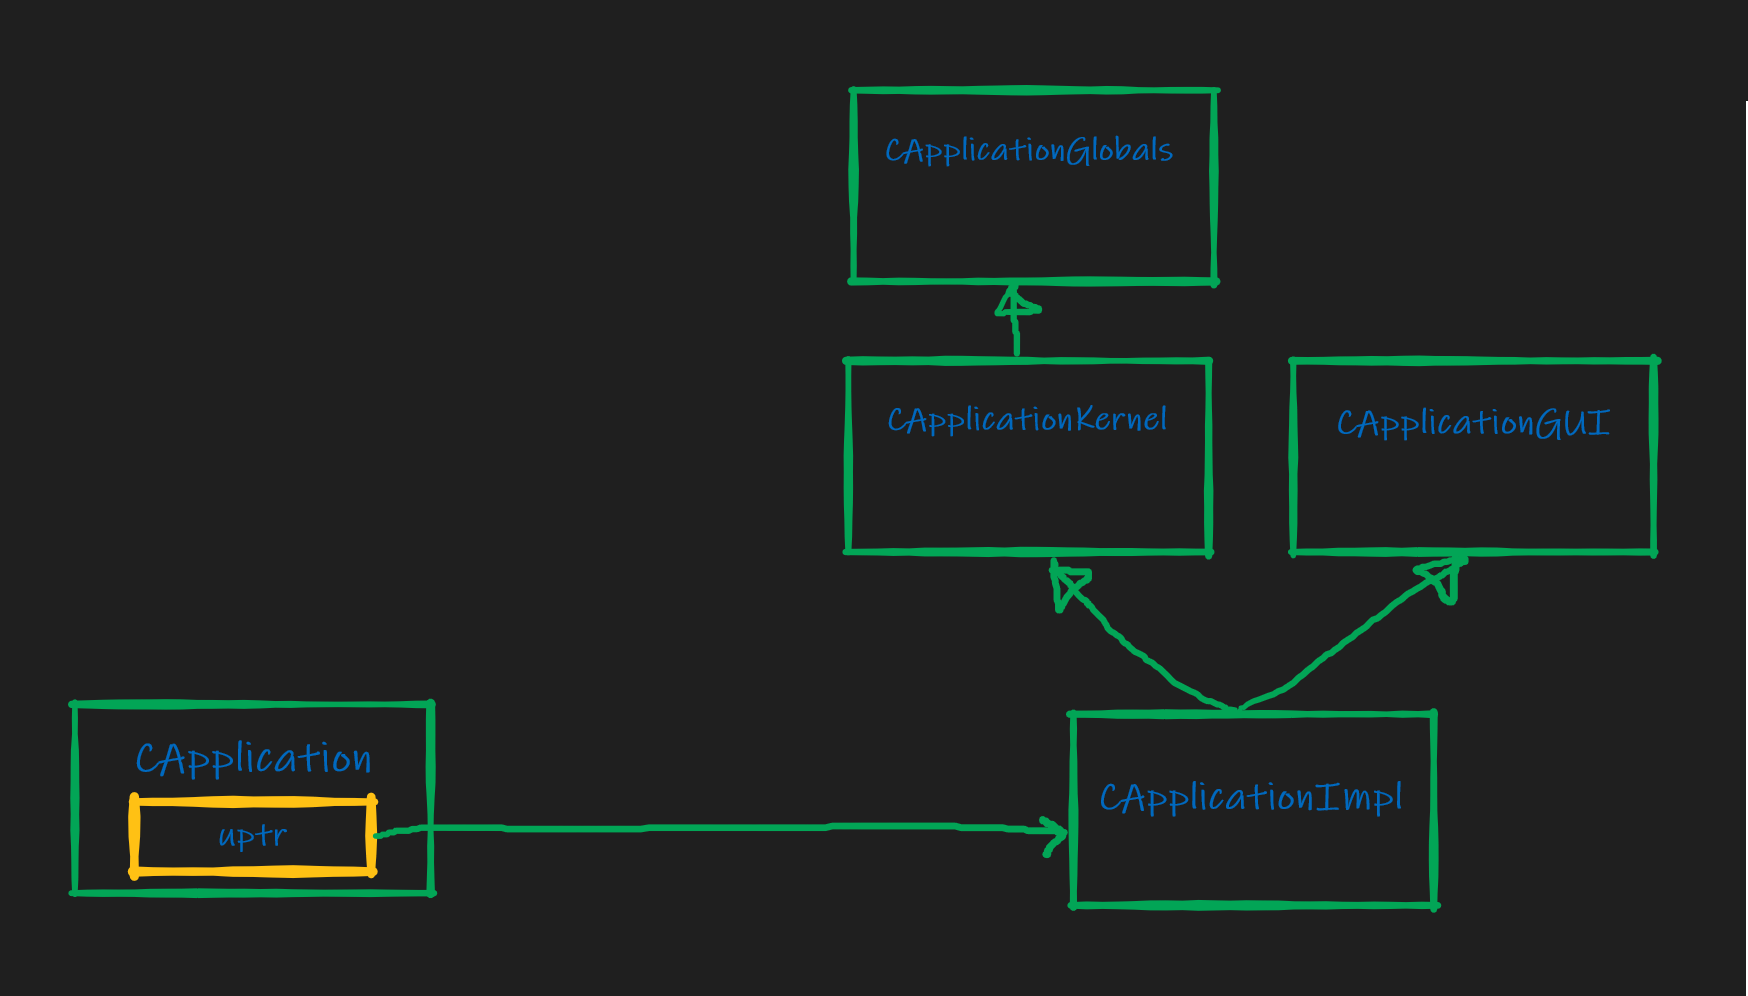
\includegraphics[scale = 0.3]{Figures/CApplicationStructure.png}
\end{center}

\subsection{Keyboard}

Each key on a keyboard has its position identifier \verb"CKeyPosition" and a key identifier \verb"CKeyId" (TO DO not implemented). CKeyPosition points out a physical location on a keyboard (e.g. a row and a column where the key is located). CKeyId identify the key depending on the keyboard layout (qwerty, Dvorak, etc.) CKeyPosition is an enum with following identifiers (xkb identifiers):
\begin{center}
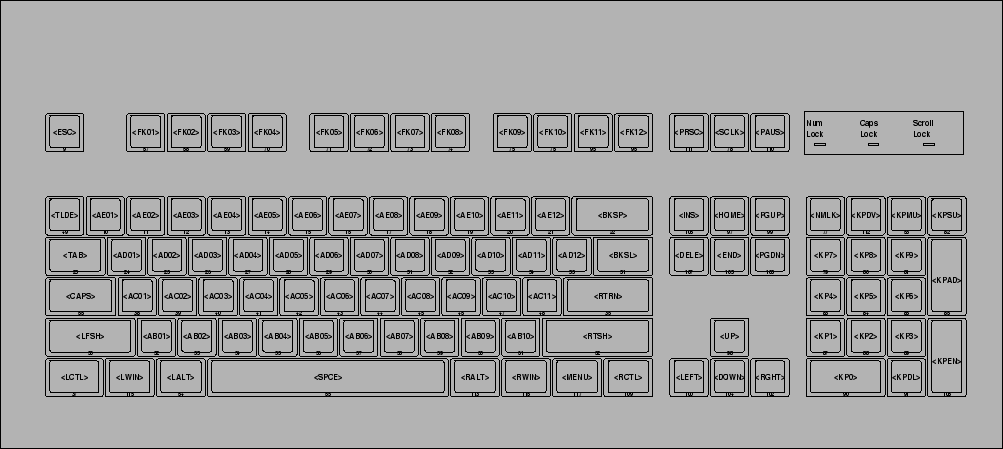
\includegraphics[scale = 0.5]{Figures/KeyPosition.png}

The picture is taken from \href{https://www.charvolant.org/doug/xkb/html/node5.html}{here}
\end{center}
It should be noted that the numeric values of the identifiers are slightly different from the one in xkb.

\subsection{Global Objects}

\subsubsection{Timer}

Application uses one main timer. This is a singleton with respect to the template here~\ref{section::Singleton}. It starts in the constructor of CApplicationGlobal. Timer return CTime object. It does not depend on particular units but you may convert it to any units you want. Internally \verb"std::chrono" is used.

\subsubsection{KeyboardHandler}

Application uses CKeyboardHandler object to intercept keyboard system-wise, that is, it intercepts the keyboard even if application is not in the focus. Qt does not support such functionality. Thus the corresponding mechanism is implemented.

CKeyboardHandler is wrapper into a singleton according to Section~\ref{section::Singleton}. It is initialized in CApplicationGlobal. From the user point of view CKeyboardHandler able to send the following information to the application objects:
\begin{enumerate}
\item \textbf{CRawKeyEvent}. This is a system independent representation of a keyboard event (TO DO currently not implemented). This event is sent via Observer pattern (TO DO currently not implemented).

\item \textbf{CQtException}. This is a message with information about an exception encountered. CKeyboardHandler sends a Qt signal to CQtLoopExceptionHandler with the corresponding CQtException object. The application terminates on any exception.
\end{enumerate}

Interception of the keyboard is implemented as follows. CKeyboardHandler spans a worker thread with OS dependent message loop. There are two objects operate on the worker thread:
\begin{enumerate}
\item \textbf{CKeyboardListener}. This object starts an OS dependent event loop with exec() function. It listen to two type of messages:
\begin{enumerate}
\item OS key events.
\item CKeyboardHandler stop event.
\end{enumerate}
CKeyboardListener intercepts any key events in OS, transform system dependent key events into CRawKeyEvent-s (TO DO currently not implemented), and sends the events to CKeyboardHandler. If stop event is encountered the event loop on the worker thread is terminated and the thread stops.

\item \textbf{CListenerExceptionHandler}. This object intercepts any exceptions on the working thread, transforms the excetions to CQtException-s, and sends them to CKeyboardHandler. If an exception is encountered the event loop is terminated and the worker thread stops.
\end{enumerate}

CKeyboardListener is OS dependent. Currently support for Windows, MacOS, and Linux is provided (TO DO only Windows listener is implemented). In order to send the Stop signal in and OS independent fashion the application uses CAnyKeyboardKiller object. It is based on CAnyMoveable object as described in~\ref{section::AnyMovable}.

\begin{center}
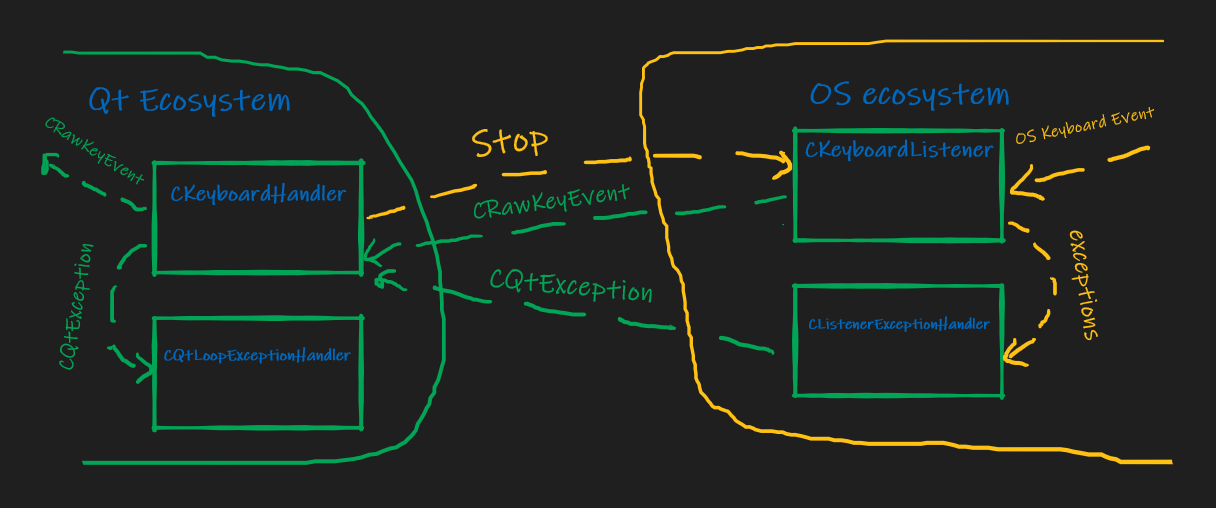
\includegraphics[scale = 0.5]{Figures/KeyboardInterception.png}

Green arrows represent queued Qt signals and yellow arrows represent OS dependent signals.
\end{center}

\subsection{Kernel}

\subsection{Qt Resources}

\subsection{ApplicationImpl}


\section{Code}

\section{Implementation}

\section{Library}
\subsection{Singleton}\label{section::Singleton}
CAnyGlobalAccess template consists of three parts:
\begin{enumerate}
\item \textbf{CAnyGlobalAccessible}. It provides a static storage for a global object. You do not access it directly.
\item \textbf{CAnyGlobalAccess}. This object is used to access the global object. The global object must be initialized before access object is created.
\item \textbf{CAnyGlobalInitializer}. This object is used to initialize the global object. You need to create one instance of this object in order to initialize the global object.
\end{enumerate}
\begin{center}
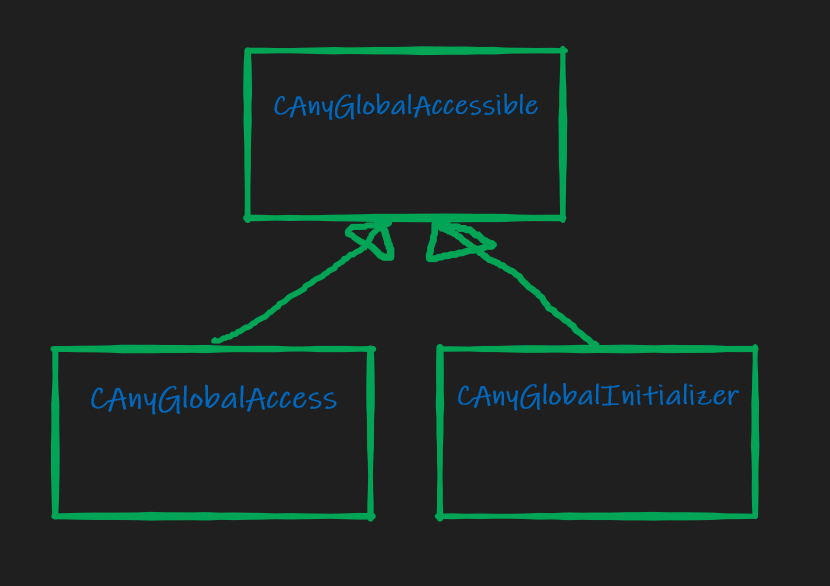
\includegraphics[scale = 0.3]{Figures/CAnyGlobalAccess.png}
\end{center}

\paragraph{Description}
The pattern is used to make a global object with non-trivial constructor without explicitly defining the object globally. \textbf{WARNING} this thing is NOT thread safe! In order to use the pattern we must provide:
\begin{enumerate}
\item \verb"TAccessible" -- the class for the global object

\item \verb"TID" -- identification class. If we want to have several global objects  of a class Type, we must distinguish them by a dummy class \verb"TID". For example, \verb"CAnyGlobalAccessible<Type, A>" and \verb"CAnyGlobalAccessible<Type, B>" store  different instances of objects of type Type in static storage. Since static objects defined by the class they belong to, classes \verb"A" and \verb"B" are required to distinguish the instances.

Example of a dummy class declaration:
\begin{verbatim}
class CGlobalAccessibleID;
\end{verbatim}

\item A class for initialization of the global object. It must be
 inherited from \verb"CAnyGlobalInitializer". The class must inherit all the constructors of the base class.
\begin{verbatim}
class CMyInitializer : CAnyGlobalInitializer<TAccessible, TID> {
   using CBase = CAnyGlobalInitializer<TAccessible, TID>;
 public:
   using CBase::CBase;
 };
\end{verbatim}

\item A class for getting access to the global object must be publicly inherited from \verb"CAnyGlobalAccess". It has only a default constructor. It asserts if  the global object has not yet been initialized.
\begin{verbatim}
class CMyAccessor : public CAnyGlobalAccess<TAccessible, TID> {};
 \end{verbatim}
\end{enumerate}

\paragraph{Example}
Suppose we want a global \verb"int" variable for logging:
\begin{verbatim}
class CLoggerCounterID;
class CLoggerCounterInitializer :
  CAnyGlobalInitializer<int, CLoggerCounterID> {
  using CBase = CAnyGlobalInitializer<int, CLoggerCounterID>;
public:
  using CBase::CBase;
};
class CLoggerCounterAccess : public CAnyGlobalAccess<int, CLoggerCounterID> {};
\end{verbatim}
Then in code we write something like that:
\begin{verbatim}
...
CLoggerCounterInitializer Init(0);
...
CLoggerCounterAccess LogCounter;
++(*LogCounter);
std::cout << *LogCounter << std::endl;
...
\end{verbatim}

\subsection{AnyObject}
\subsubsection{AnyMovable}\label{section::AnyMovable}

\paragraph{Description}
\verb"CAnyMovable" allows you to store any movable only class without any restrictions on the class. It also allows you to provide  an interface to a class and implementations for different classes of the method.

The \verb"operator->()" goes without any checks and may fail if the object is empty, that is, does not store anything. It is your responsibility to call \verb"isDefined()" method before accessing the interface.

The class \verb"CAnyMovable" does not use Small Object Optimization. In particular, move operations are always cheap. \verb"CAnyMovable" has value semantics and extends the ideas of Sean Parent's talk on cppcon about Run-time Polymorphism.

\paragraph{How to use}
In order to use the template you need:
\begin{enumerate}
\item Create an interface class:
\begin{verbatim}
template<class TBase>
class IAny : public TBase {
public:
  virtual void print() const = 0;
};
\end{verbatim}
The class describes the interface of an abstract object you want to support. Do not use names with prefix underscore here, e.g.,
\begin{itemize}
\item[\textbf{BAD}:] \verb"virtual void _print() const = 0;"
\item[\textbf{GOOD}:] \verb"virtual void print() const = 0;"
\end{itemize}
This interface will be accessible when using \verb"operator->()" on \verb"CAnyObject". The example is below.

\item Create an implementation class:
\begin{verbatim}
template<class TBase, class TObject>
class CAnyImpl : public TBase {
  using CBase = TBase;
public:
  using CBase::CBase;
  void print() const override {
    std::cout << "data = " << CBase::Object() << std::endl;
  }
};
\end{verbatim}
Here you implement all the functions from the interface. The parameter \verb"TObject" is used to reimplement the behaviour for different types of objects if needed. In the example above, it may happen that \verb"TObject" does not support stream \verb"operator<<" and you want to define  a specialization of the implementation class. Access to the stored object is provided by the method \verb"CBase::Object()".

\item Create your Any class:
\begin{verbatim}
class CAny : public CAnyMovable<IAny, CAnyImpl> {
  using CBase = CAnyMovable<IAny, CAnyImpl>;
public:
  using CBase::CBase;
  friend bool operator==(const CAny&, const CAny&) {
    ...
  }
};
\end{verbatim}
You can add any additional functionality to your \verb"CAny" class.
\end{enumerate}
Now you can use it like this:
\begin{verbatim}
CAny x = 'c';
x->print();
x = std::move("123");
x->print();
x = 1.45;
x->print();
\end{verbatim}
If you want to store an object of Type \verb"R" and construct it on the fly from the data: \verb"x, y, z". Then use emplace function or emplace constructor like this:
\begin{verbatim}
CAny s;
s.emplace<R>(x, y, z);
CAny y(std::in_place_type_t<R>(), x, y, z);
\end{verbatim}
Then the object of type \verb"R" will be created without creation of intermediate objects.

\paragraph{Implementation}
Internally \verb"CAnyMovable" stores an \verb"std::unique_ptr" to interface \verb"IObjectStored". Let us look at the diagram below:
\begin{center}
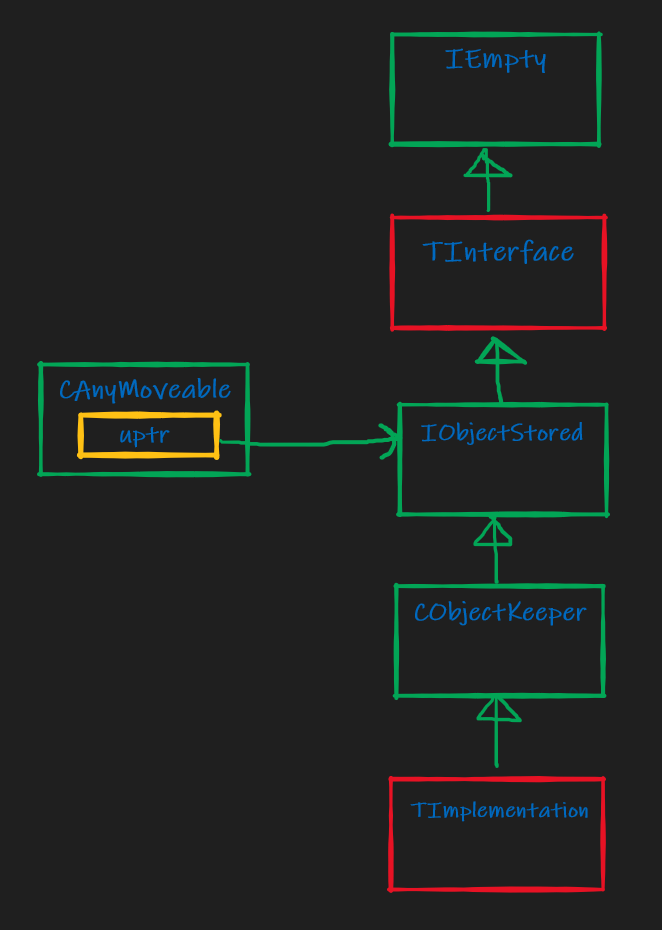
\includegraphics[scale = 0.5]{Figures/CAnyMovable.png}
\end{center}
The red rectangles are templates provided by the user. \verb"IEmpty" is an empty interface with virtual distructor. Its only purpose is to avoid user having to provide a virtual distructor in the \verb"TInterface" template. Then \verb"IObjectStored" adds some virtual methods to provide required functionality. \verb"CObjectKeeper" is a template storing an instance of an object you want to move into \verb"CAnyMovable". \verb"TImplementation" is a user defined template implementing all virtual methods from \verb"TInterface".

\end{document}


